
\documentclass[a4paper,12pt]{article}

\usepackage[utf8]{inputenc}
\usepackage[T1]{fontenc}
\usepackage{geometry}
\usepackage{graphicx}
\usepackage{url}

\renewcommand{\refname}{Viri}


\geometry{margin=2.5cm}

\begin{document}

\begin{titlepage}
    \centering
    
    \vfill
    
    {\large }


    {\Huge \textbf{SN\&US}}\\[0.3cm]
    {\large Simply New \& United Security}

    \vspace{2cm}

    {\LARGE \textbf{Pregled obstoječih rešitev}}\\[0.5cm]

    {\large Analiza primerljivih rešitev
    na področju kibernetske varnosti}

    \vfill

    \textbf{Ekipa:}\\
    Žan Vidovič\\
    Marcel Smolar

    \vfill

    Maribor \\ November 2026

\end{titlepage}
% prva stran je tu fertik ================================================

\section{}\large{{\textbf{Uvod}}


Ciljna ideja najine teme je bil \textbf{Cyber-Security}, bolj natančno je bilo področje kibernetske varnosti za obrambo proti napadom, odziv na incident in beleženje vseh poskušenih vdorov v sisteme.\\
\\
Vedno hitreje postaja kibernetska varnost resničen izziv za veliko podjetij, saj vsi pogosto uporabljamo enaka gesla, ne razmišljamo preveč preden kliknemo na kakršenkoli link, z veseljem nalagamo brezplačen RAM in še katerekoli druge bedarije. Ta problem je postal tako pogost, da se v skupinah ljudje včasih o tem celo zabavajo, ne da bi se zavedali da ves čas riskirajo svoje podatke, zato je SN\&US namenjen avtomatizirani zaščiti, ki lahko reši še najbolj gullible podjetja.

\break

%=================================================================================

\section{IBM -- Cyberthreat Management Services}

IBM je mednarodno tehnološko podjetje, ki ponuja tudi številne storitve na področju kibernetske varnosti. Njihova rešitev Cyberthreat Management Services združuje preventivno zaščito, zaznavanje groženj in odzivanje na varnostne incidente.\cite{ibm}

\subsection{Ključne funkcionalnosti}

\begin{itemize}
    \item \textbf{Zaznavanje groženj:} spremljanje sistemov in prepoznavanje sumljivih aktivnosti.
    \item \textbf{Odzivanje na incidente:} pomoč pri obravnavi varnostnih incidentov.
    \item \textbf{Obveščevalni podatki:} analiziranje novih groženj in tehnik napadalcev.
\end{itemize}

\subsection{Prednosti}

\begin{itemize}
    \item Širok nabor varnostnih storitev.
    \item Kombinacija strokovnega znanja in avtomatiziranih orodij.
    \item Podpora pri preprečevanju napadov in odzivanju nanje.
\end{itemize}

\subsection{Slabosti}

\begin{itemize}
    \item Veliko število storitev lahko oteži orientacijo neizkušenim uporabnikom.
    \item Ponudba je lahko preobsežna za manjša podjetja.
\end{itemize}

\begin{figure}[b!]
    \centering
    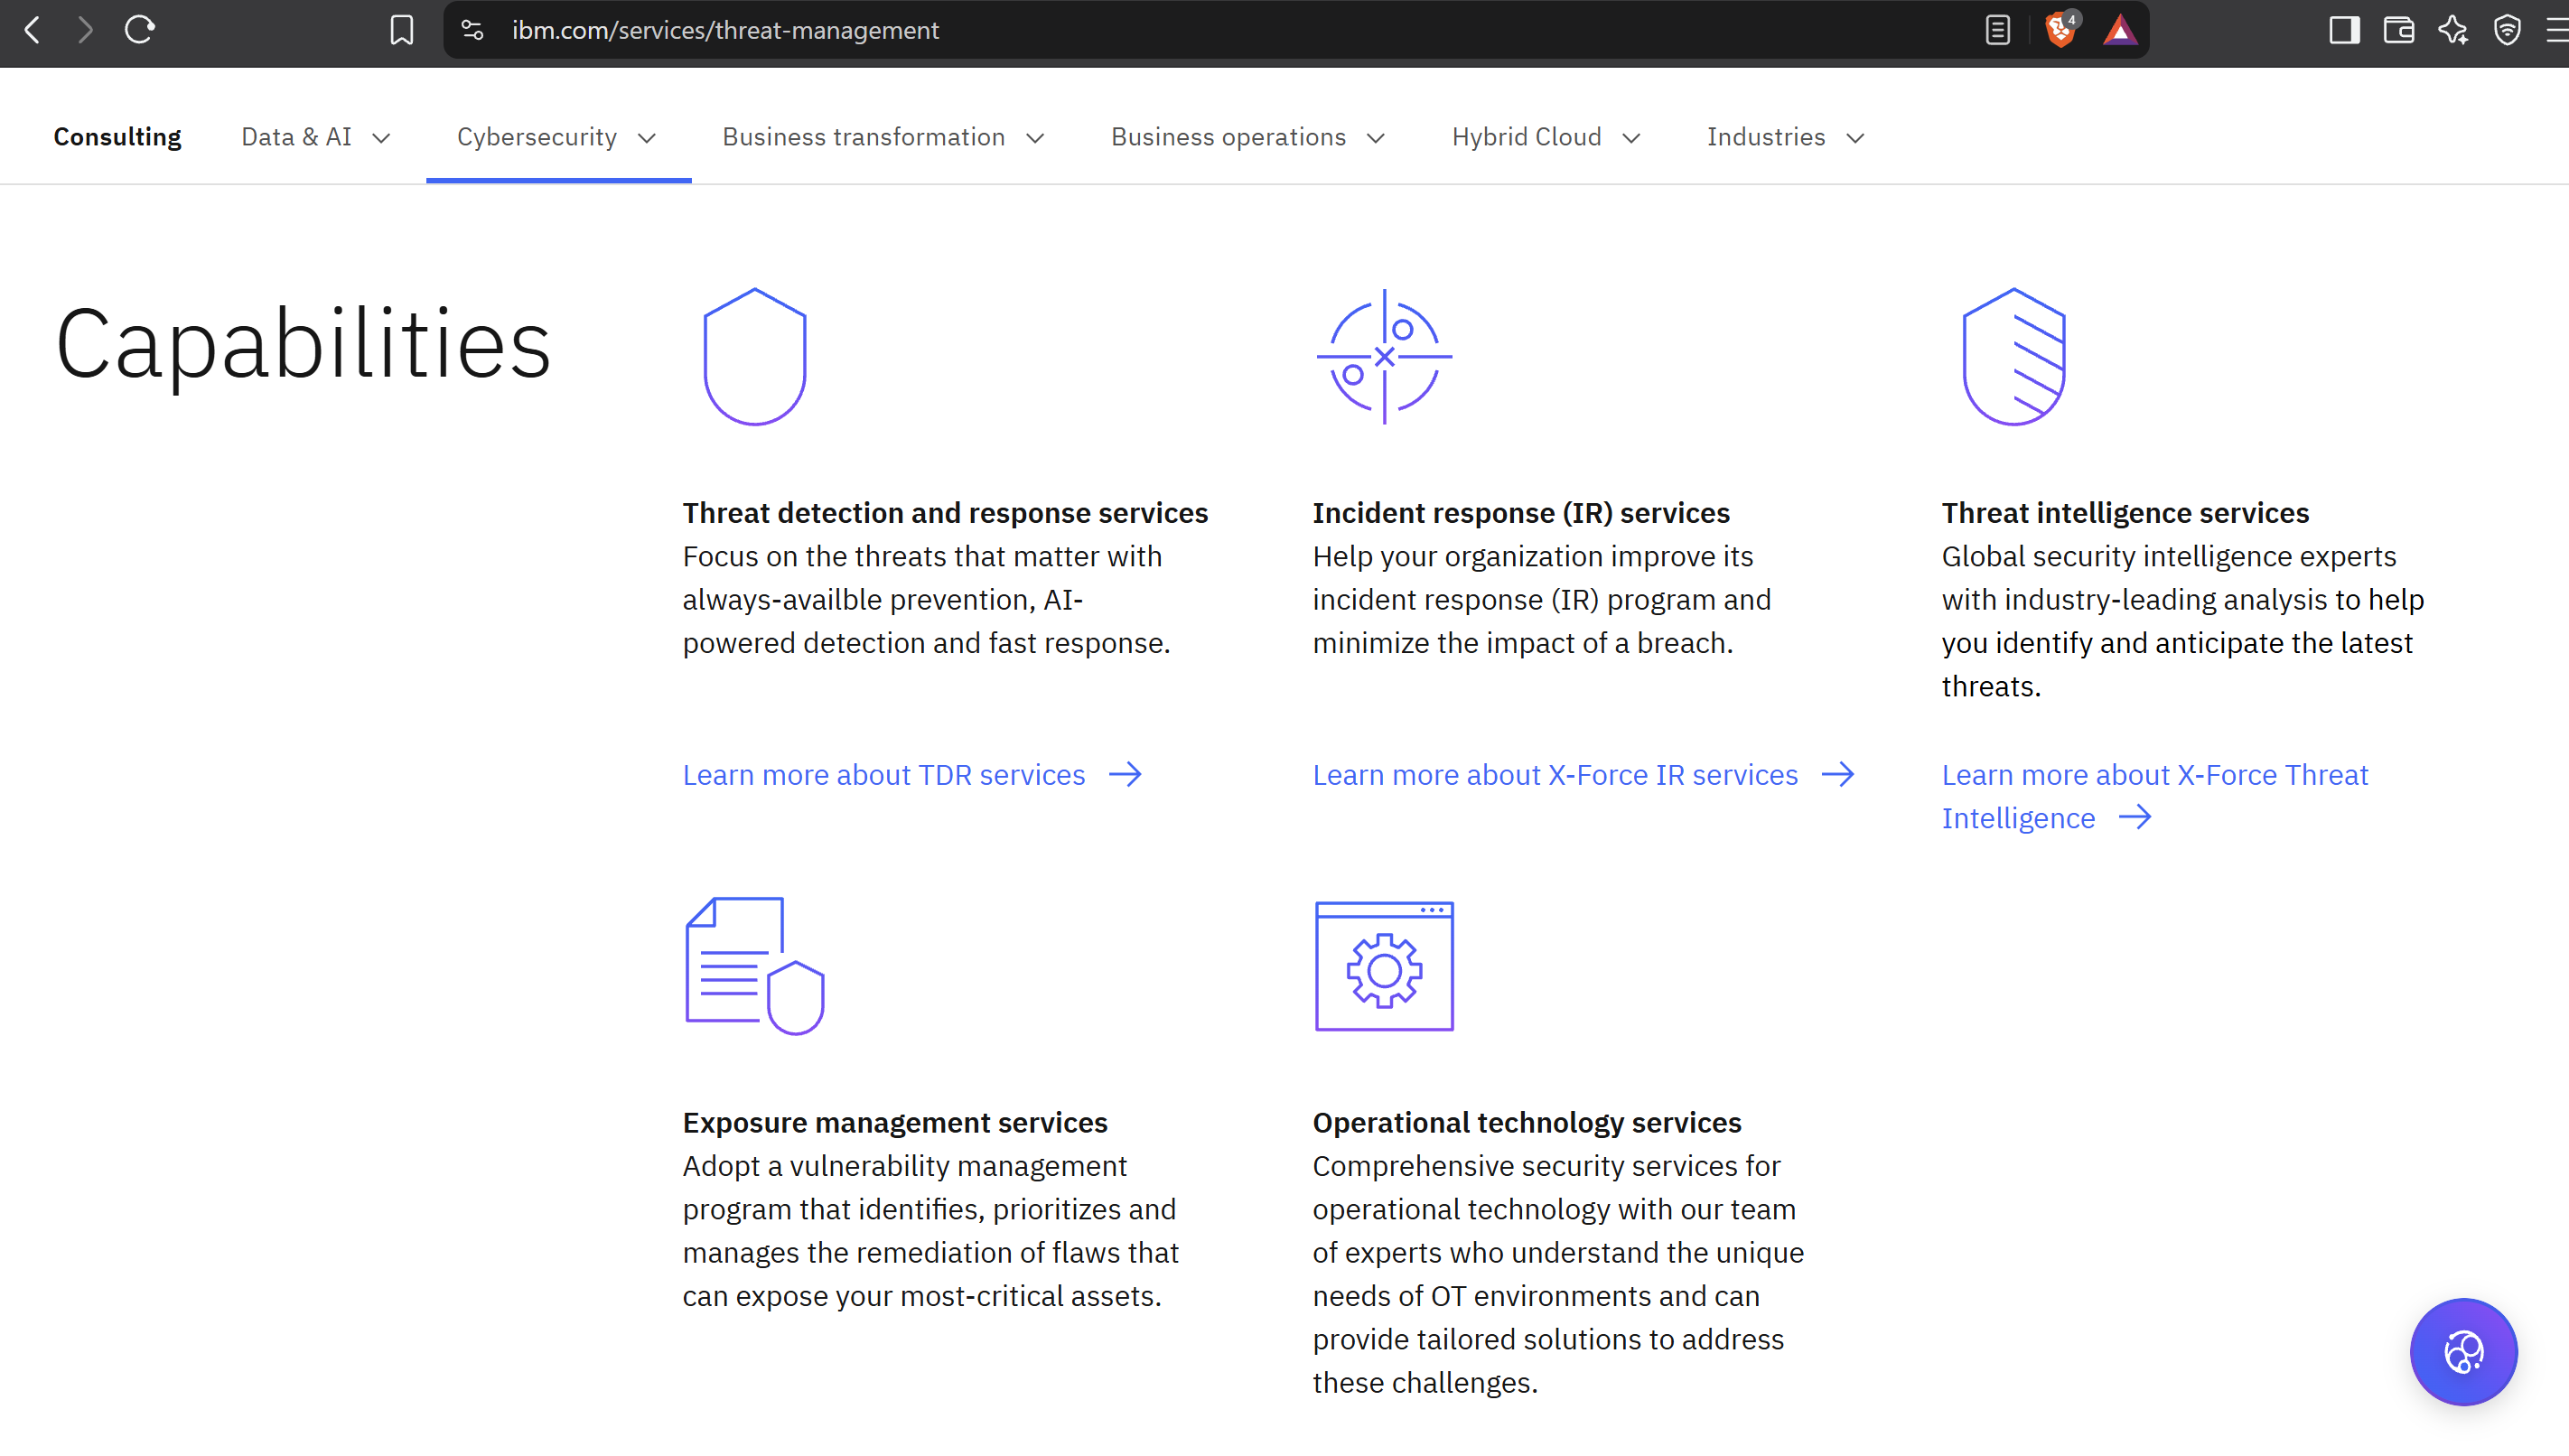
\includegraphics[width=0.6\linewidth]{ibm-cms.png}
    \caption{Pregled varnostnih storitev podjetja IBM}
    \label{fig:ibm-cms}
\end{figure}

\break


%===============================================================================

\section{Sophos -- Ransomware Protection}

Sophos je podjetje, specializirano za razvoj rešitev na področju kibernetske varnosti. Njihova rešitev Ransomware Protection je namenjena preprečevanju izsiljevalskih napadov, zaščiti naprav in hitremu odzivanju na zaznane grožnje.
\cite{sophos}

\subsection{Ključne funkcionalnosti}

\begin{itemize}
    \item \textbf{Zaščita končnih naprav:} preprečevanje zlonamernih aktivnosti na računalnikih in strežnikih.
    \item \textbf{Zaznavanje groženj:} prepoznavanje sumljivih aktivnosti s pomočjo umetne inteligence.
    \item \textbf{Zaščita pred izsiljevalsko programsko opremo:} tehnologija CryptoGuard zazna zlonamerno šifriranje in omogoča povrnitev prizadetih datotek.
\end{itemize}

\subsection{Prednosti}

\begin{itemize}
    \item Neprekinjeno spremljanje in hitro odzivanje na grožnje.
    \item Kombinacija avtomatizirane zaščite in strokovnega nadzora.
\end{itemize}

\subsection{Slabosti}

\begin{itemize}
    \item Celovita zaščita zahteva uporabo večih Sophosovih produktov.
    \item Napredne storitve zahtevajo razumevanje varnostnih orodij.
\end{itemize}

\begin{figure}[b!]
    \centering
    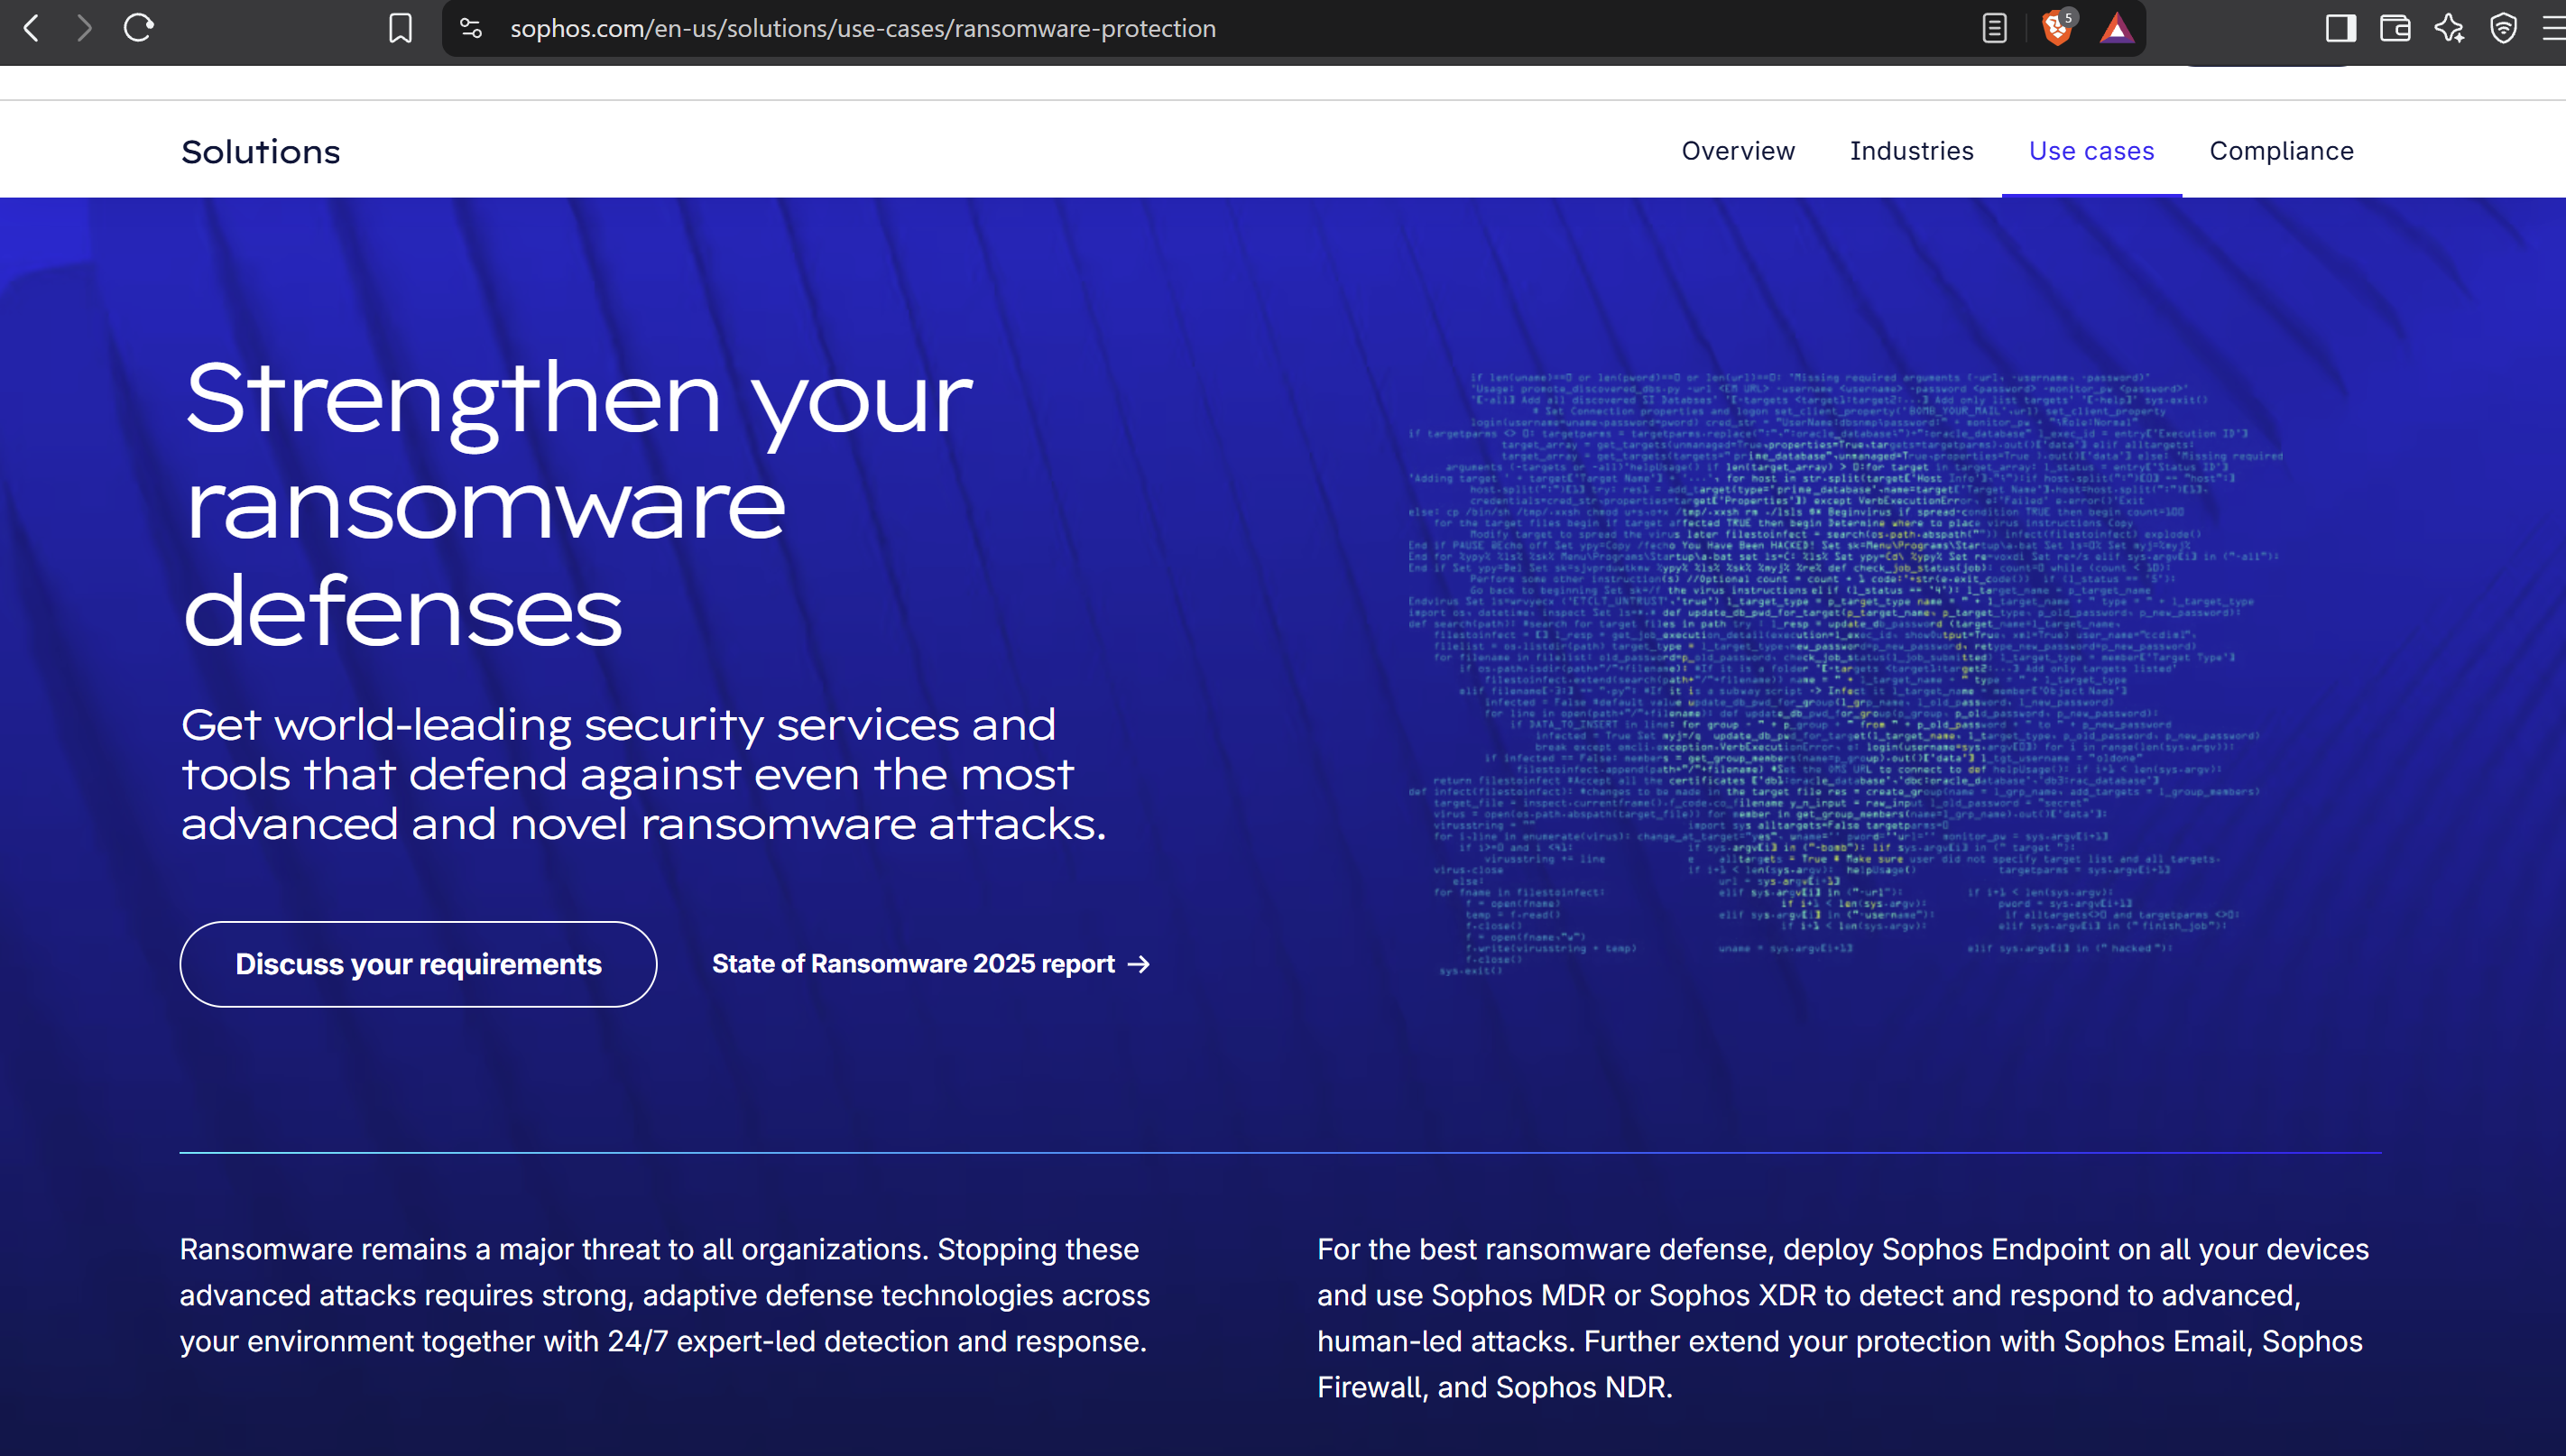
\includegraphics[width=0.6\textwidth]
    {sophos.png}
    \caption{Predstavitev rešitve Ransomware Protection podjetja Sophos}
    \label{fig:sophos}
\end{figure}

%=================================================================================


\section{NCC Group -- Cybersecurity Solutions}

NCC Group je mednarodno podjetje, specializirano za kibernetsko varnost in svetovanje. Ponuja širok nabor rešitev za zaščito digitalne infrastrukture, upravljanje varnostnih tveganj in izboljšanje odpornosti organizacij na kibernetske napade. \cite{ncc}

\subsection{Ključne funkcionalnosti}

\begin{itemize}
    \item \textbf{Varnost v oblaku:} zaščita in preverjanje varnosti oblačnih okolij.
    \item \textbf{Upravljanje identitet:} nadzor dostopa uporabnikov do sistemov in podatkov.
    \item \textbf{Proaktivna varnost:} prepoznavanje ranljivosti s pomočjo varnostnih testiranj.
\end{itemize}

\subsection{Prednosti}

\begin{itemize}
    \item Zelo širok nabor specializiranih varnostnih storitev.
    \item Možnost prilagajanja rešitev različnim organizacijam.
    \item Pokrivanje tako preventivne zaščite kot odzivanja na incidente.
\end{itemize}

\subsection{Slabosti}

\begin{itemize}
    \item Velika izbira storitev lahko oteži izbiro ustrezne rešitve.
    \item Široka ponudba zahteva več predhodnega razumevanja kibernetske varnosti.
\end{itemize}

\begin{figure}[h]
    \centering
    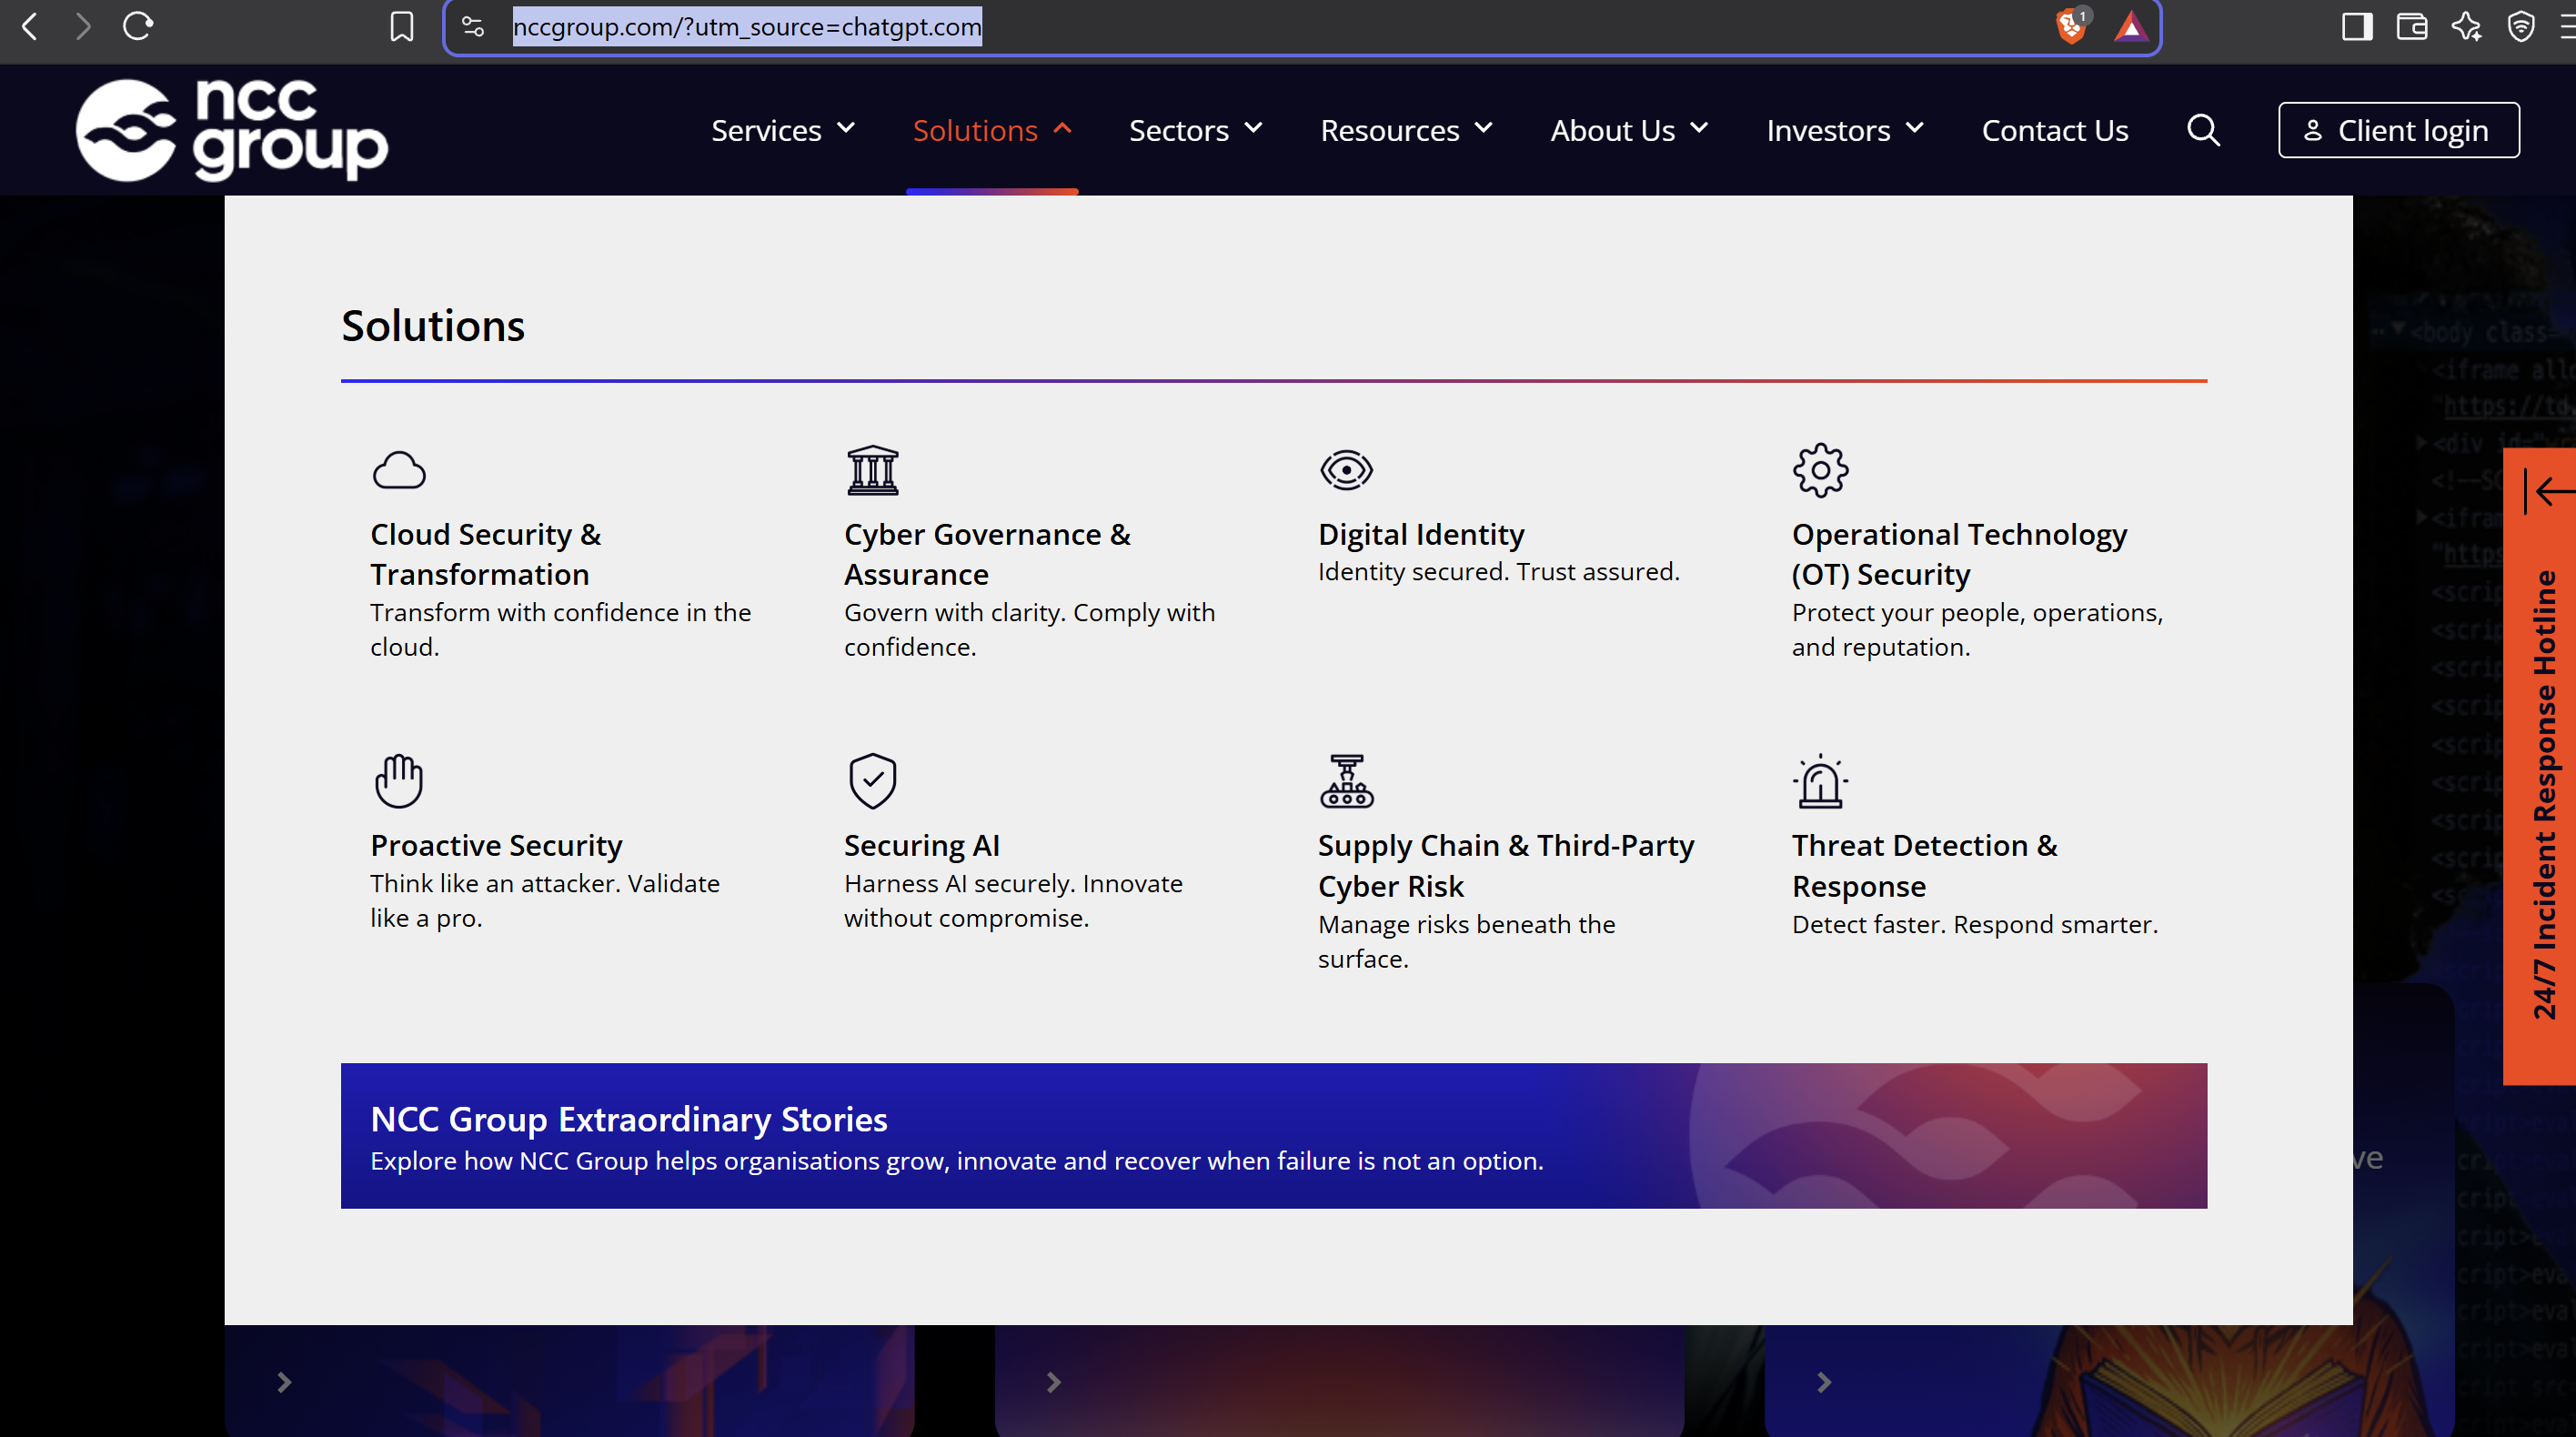
\includegraphics[width=0.6\textwidth]
    {ncc.png}
    \caption{Pregled področij kibernetske varnosti podjetja NCC Group}
    \label{fig:ncc}
\end{figure}


%=================================================================================


\section{Zaključek}

Na podlagi pregleda obstoječih rešitev smo ugotovili, da podjetja na področju kibernetske varnosti ponujajo številne načine zaščite, od zaznavanja groženj in odzivanja na incidente do zaščite naprav ter upravljanja varnostnih tveganj.\\

Pri razvoju SN\&US želimo združiti nekatere njihove najbolj uporabne pristope, vendar z nekoliko drugačnim poudarkom. Naša rešitev bo temeljila predvsem na avtomatizirani zaščiti uporabnikov in njihovih informacijskih sistemov.\\

SN\&US bo razvijal programsko opremo, namenjeno preprečevanju phishing napadov, zlonamernih prenosov, spletnih prevar in drugih oblik socialnega inženiringa. Sistem bo samodejno preverjal sumljive povezave, elektronsko pošto in datoteke ter po potrebi blokiral nevarne vsebine, še preden bi uporabnik lahko povzročil škodo.\\

Glavna prednost naše rešitve bo zmanjšanje odvisnosti od človeške previdnosti in ročnega preverjanja groženj. Namesto da bi od uporabnikov pričakovali popolno poznavanje vseh varnostnih tveganj, želimo zagotoviti dodatno zaščitno plast, ki bo nevarne aktivnosti prepoznala in preprečila samodejno.\\

Naš cilj je ustvariti čim bolj dostopno, učinkovito in zanesljivo rešitev, ki bo uporabnikom omogočala varnejšo uporabo digitalnih sistemov.

\break

%================================================================================
% citatiiiiiiii

\begin{thebibliography}{9}

\bibitem{ibm}
IBM, \textit{Cyberthreat Management Services}.
\url{https://www.ibm.com/services/threat-management}

\bibitem{sophos}
Sophos, \textit{Ransomware Protection}.
\url{https://www.sophos.com/en-us/solutions/use-cases/ransomware-protection}

\bibitem{ncc}
NCC Group, \textit{Cybersecurity Solutions}.
\url{https://www.nccgroup.com/solutions/}

\end{thebibliography}


\end{document}
